% The classical picture of one step of RK4: what a step is (from t_n to
% t_n + dt) and what its four stages are (a stage state Y_i, built from y_n and
% the previous slope, and the slope k_i = f(t_n + c_i dt, Y_i) evaluated there).
% Drawn exactly for y' = -y, y_n = 1, dt = 1, so the geometry is the real one:
%   k1 = -1     at (0,   1)
%   Y2 = 0.5,   k2 = -0.5    at t = 1/2
%   Y3 = 0.75,  k3 = -0.75   at t = 1/2
%   Y4 = 0.25,  k4 = -0.25   at t = 1
%   y_{n+1} = 1 + (k1 + 2 k2 + 2 k3 + k4)/6 = 0.375,  exact exp(-1) = 0.3679.
% Coordinates: x = 12 t, y = 8 y, in cm. Each symbol is tagged with the library
% type that holds it and the call that produces it, as the hardcoded rk4 step
% (step_rk4 in src/schemes/rk/stdlib_integrate_rk_steps.f90) does it; the key
% below the plot lists them all.
\documentclass[tikz,border=6pt]{standalone}
\usepackage{amsmath}
\usepackage{array,booktabs}
\usetikzlibrary{arrows.meta,decorations.pathreplacing,calc}

% Palette: states blue, slopes (tendencies) orange, as in rk_step_anatomy.
\definecolor{statecol}{RGB}{31,119,180}
\definecolor{tendcol}{RGB}{230,120,30}
\definecolor{exactcol}{RGB}{150,150,150}

% A library name, small, in typewriter: what holds a symbol, or what produces it.
\newcommand{\ty}[1]{\leavevmode{\footnotesize\ttfamily\color{black!65}#1}}

\begin{document}
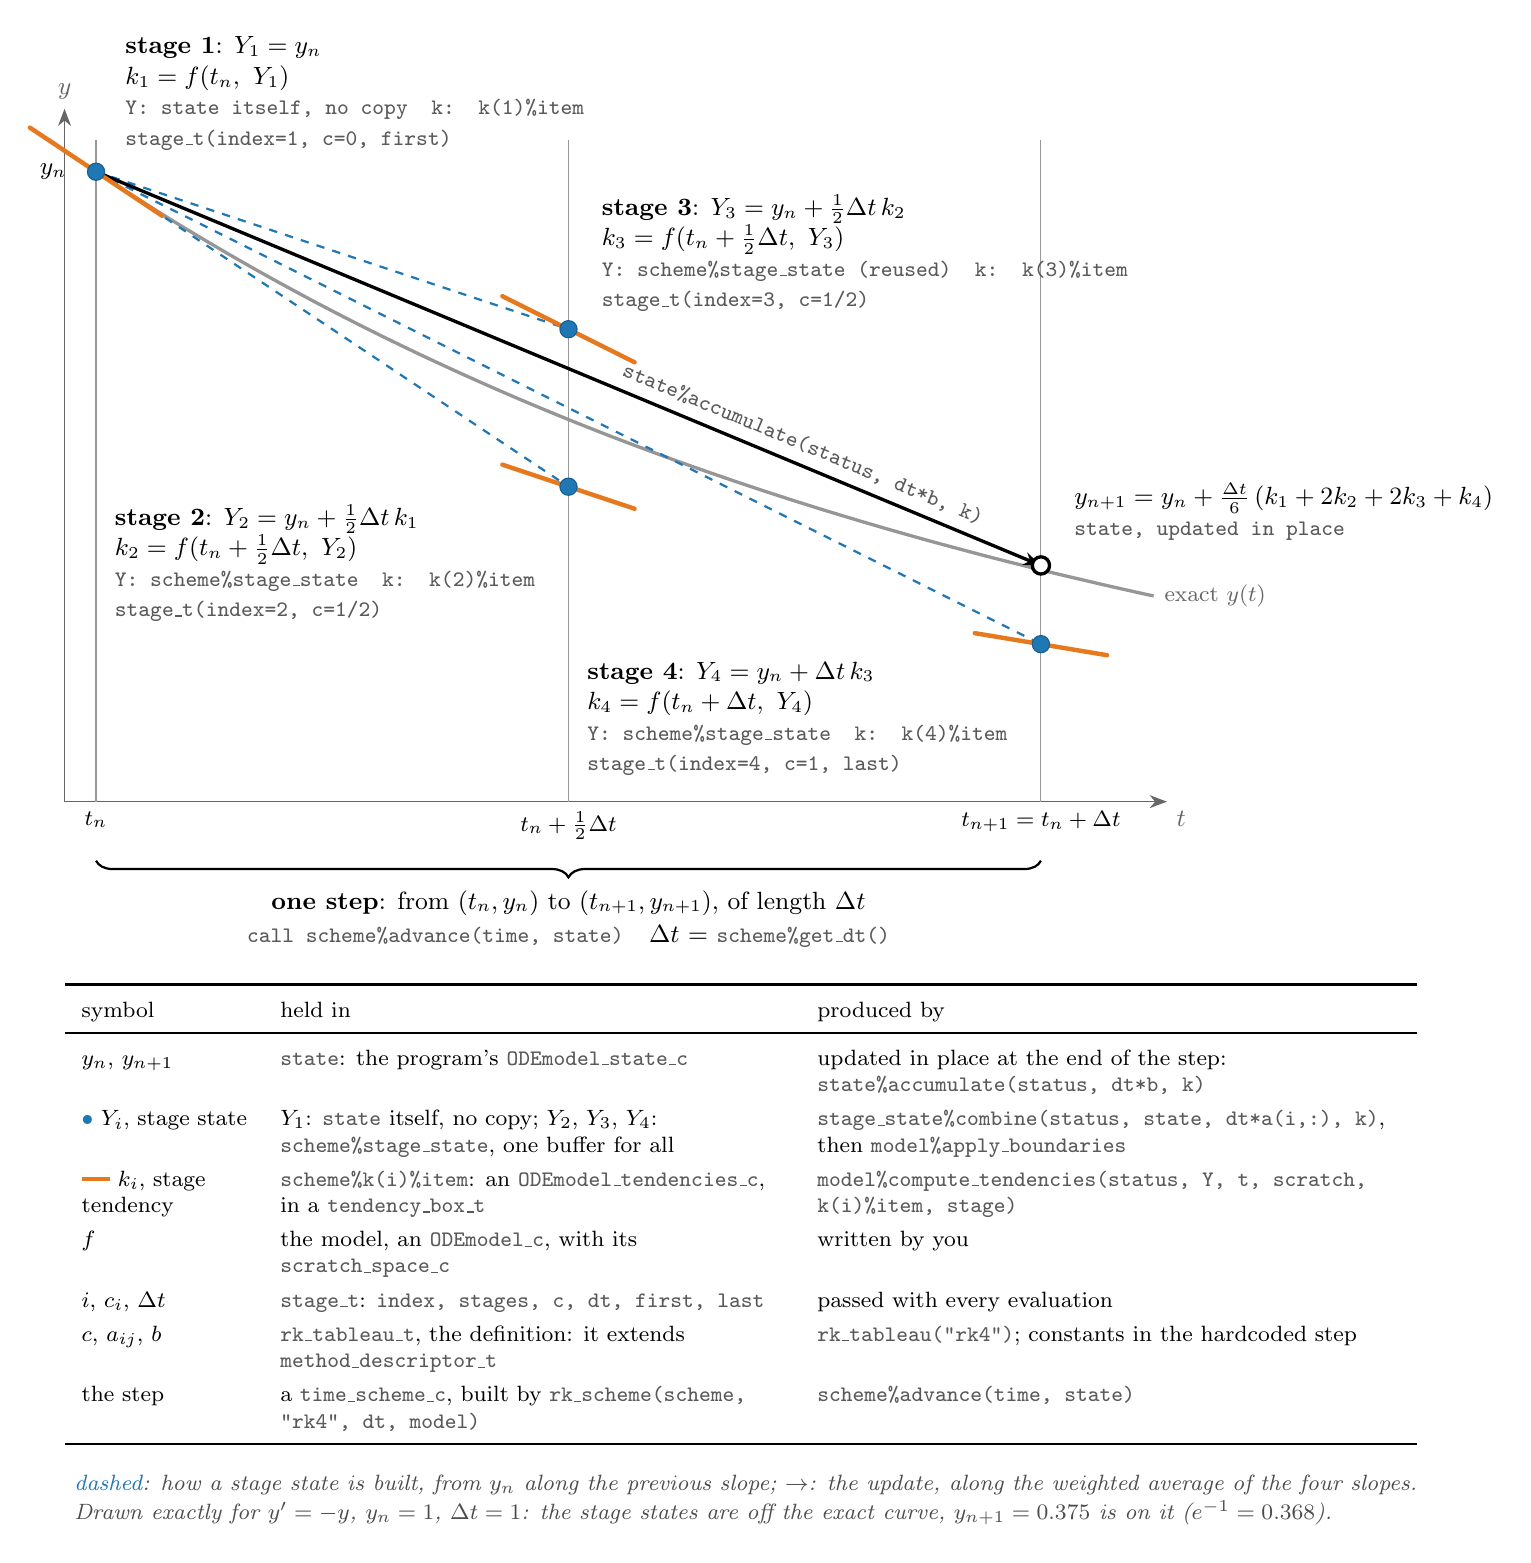
\begin{tikzpicture}[
    font=\small,
    >={Stealth[length=2.2mm]},
    state/.style={circle, draw=statecol!80!black, fill=statecol, inner sep=2.2pt},   % a stage state Y_i
    newstate/.style={circle, draw=black, fill=white, very thick, inner sep=2.2pt},    % the new state y_{n+1}
    slope/.style={tendcol, line width=1.6pt, line cap=round},                         % the slope k_i at Y_i
    build/.style={statecol, dashed, thick},                                           % how Y_i is built from y_n
    lbl/.style={font=\small, align=left},                                             % a stage label
    note/.style={font=\footnotesize\itshape, text=black!70, align=left},              % explanatory note
    ty/.style={font=\footnotesize\ttfamily, text=black!65},                          % a library name on the plot
  ]

  % ---- the data-to-picture map, x = 12 t, y = 8 y ----
  \def\X#1{12*(#1)}
  \def\Y#1{8*(#1)}

  % ---- axes ----
  \draw[->, black!60] (-0.4, 0) -- (13.6, 0) node[below right] {$t$};
  \draw[->, black!60] (-0.4, 0) -- (-0.4, 8.8) node[above] {$y$};
  \foreach \t/\name in {0/{t_n}, 0.5/{t_n + \tfrac12\Delta t}, 1/{t_{n+1} = t_n + \Delta t}} {
    \draw[black!40] ({\X{\t}}, 0) -- ({\X{\t}}, 8.4);
    \node[below, font=\footnotesize] at ({\X{\t}}, 0) {$\name$};
  }

  % ---- the step: one interval of length dt ----
  \draw[decorate, decoration={brace, mirror, amplitude=6pt}, thick]
       (0, -0.75) -- (12, -0.75) node[midway, below=7pt, align=center] {\textbf{one step}: from $(t_n, y_n)$ to $(t_{n+1}, y_{n+1})$, of length $\Delta t$\\[1pt]
       \ty{call scheme\%advance(time, state)}\quad $\Delta t$ = \ty{scheme\%get\_dt()}};

  % ---- the exact solution through y_n ----
  \draw[exactcol, very thick] plot[domain=-0.05:1.12, samples=80, smooth] ({\X{\x}}, {\Y{exp(-\x)}})
       node[right, font=\footnotesize, text=black!60] {exact $y(t)$};

  % ---- how the stage states are built: from y_n, along the previous slope ----
  \draw[build] ({\X{0}}, {\Y{1}}) -- ({\X{0.5}}, {\Y{0.5}});     % Y2 = y_n + dt/2 k1
  \draw[build] ({\X{0}}, {\Y{1}}) -- ({\X{0.5}}, {\Y{0.75}});    % Y3 = y_n + dt/2 k2
  \draw[build] ({\X{0}}, {\Y{1}}) -- ({\X{1}},   {\Y{0.25}});    % Y4 = y_n + dt   k3

  % ---- the update: from y_n, along the weighted average of the slopes ----
  \draw[black, very thick, ->] ({\X{0}}, {\Y{1}}) -- ({\X{1}}, {\Y{0.375}})
       node[pos=0.74, sloped, above, ty] {state\%accumulate(status, dt*b, k)};

  % ---- the slopes evaluated at each stage state (short tangent segments) ----
  \foreach \t/\y/\k in {0/1/-1, 0.5/0.5/-0.5, 0.5/0.75/-0.75, 1/0.25/-0.25} {
    \draw[slope] ({\X{\t - 0.07}}, {\Y{\y - 0.07*(\k)}}) -- ({\X{\t + 0.07}}, {\Y{\y + 0.07*(\k)}});
  }

  % ---- the stage states and the new state ----
  \node[state]    (Y1) at ({\X{0}},   {\Y{1}})     {};
  \node[state]    (Y2) at ({\X{0.5}}, {\Y{0.5}})   {};
  \node[state]    (Y3) at ({\X{0.5}}, {\Y{0.75}})  {};
  \node[state]    (Y4) at ({\X{1}},   {\Y{0.25}})  {};
  \node[newstate] (yn1) at ({\X{1}},  {\Y{0.375}}) {};

  % ---- stage labels ----
  \node[lbl, anchor=south west] at ($(Y1)+(0.25, 0.15)$)
       {\textbf{stage 1}: $Y_1 = y_n$\\ $k_1 = f(t_n,\ Y_1)$\\
        \ty{Y: state itself, no copy\quad k: k(1)\%item}\\ \ty{stage\_t(index=1, c=0, first)}};
  \node[lbl, anchor=north east] at ($(Y2)+(-0.3, -0.1)$)
       {\textbf{stage 2}: $Y_2 = y_n + \tfrac12\Delta t\, k_1$\\ $k_2 = f(t_n + \tfrac12\Delta t,\ Y_2)$\\
        \ty{Y: scheme\%stage\_state\quad k: k(2)\%item}\\ \ty{stage\_t(index=2, c=1/2)}};
  \node[lbl, anchor=south west] at ($(Y3)+(0.3, 0.1)$)
       {\textbf{stage 3}: $Y_3 = y_n + \tfrac12\Delta t\, k_2$\\ $k_3 = f(t_n + \tfrac12\Delta t,\ Y_3)$\\
        \ty{Y: scheme\%stage\_state (reused)\quad k: k(3)\%item}\\ \ty{stage\_t(index=3, c=1/2)}};
  \node[lbl, anchor=north east] at ($(Y4)+(-0.3, -0.1)$)
       {\textbf{stage 4}: $Y_4 = y_n + \Delta t\, k_3$\\ $k_4 = f(t_n + \Delta t,\ Y_4)$\\
        \ty{Y: scheme\%stage\_state\quad k: k(4)\%item}\\ \ty{stage\_t(index=4, c=1, last)}};
  \node[lbl, anchor=south west] at ($(yn1)+(0.3, 0.2)$)
       {$y_{n+1} = y_n + \tfrac{\Delta t}{6}\,(k_1 + 2k_2 + 2k_3 + k_4)$\\ \ty{state, updated in place}};
  \node[font=\small, anchor=east, align=right] at ($(Y1)+(-0.25, 0)$) {$y_n$};

  % ---- key: each symbol, what holds it in the library, what produces it ----
  \node[anchor=north west, font=\footnotesize, inner sep=0pt] (key) at (-0.4, -2.3) {%
    \renewcommand{\arraystretch}{1.3}%
    \begin{tabular}{>{\raggedright}p{2.1cm} >{\raggedright}p{6.4cm} >{\raggedright\arraybackslash}p{7.4cm}}
      \toprule
      symbol & held in & produced by \\
      \midrule
      $y_n$, $y_{n+1}$ & \ty{state}: the program's \ty{ODEmodel\_state\_c} &
        updated in place at the end of the step: \ty{state\%accumulate(status, dt*b, k)} \\
      \textcolor{statecol}{$\bullet$} $Y_i$, stage state & $Y_1$: \ty{state} itself, no copy; $Y_2$, $Y_3$, $Y_4$: \ty{scheme\%stage\_state}, one buffer for all &
        \ty{stage\_state\%combine(status, state, dt*a(i,:), k)}, then \ty{model\%apply\_boundaries} \\
      \textcolor{tendcol}{\rule[0.5ex]{1.2em}{1.6pt}} $k_i$, stage tendency & \ty{scheme\%k(i)\%item}: an \ty{ODEmodel\_tendencies\_c}, in a \ty{tendency\_box\_t} &
        \ty{model\%compute\_tendencies(status, Y, t, scratch, k(i)\%item, stage)} \\
      $f$ & the model, an \ty{ODEmodel\_c}, with its \ty{scratch\_space\_c} & written by you \\
      $i$, $c_i$, $\Delta t$ & \ty{stage\_t}: \ty{index, stages, c, dt, first, last} & passed with every evaluation \\
      $c$, $a_{ij}$, $b$ & \ty{rk\_tableau\_t}, the definition: it extends \ty{method\_descriptor\_t} & \ty{rk\_tableau("rk4")}; constants in the hardcoded step \\
      the step & a \ty{time\_scheme\_c}, built by \ty{rk\_scheme(scheme, "rk4", dt, model)} & \ty{scheme\%advance(time, state)} \\
      \bottomrule
    \end{tabular}};
  \node[note, anchor=north west] at ($(key.south west)+(0, -0.25)$)
       {\textcolor{statecol}{dashed}: how a stage state is built, from $y_n$ along the previous slope;
        \textbf{$\rightarrow$}: the update, along the weighted average of the four slopes.\\[1pt]
        Drawn exactly for $y' = -y$, $y_n = 1$, $\Delta t = 1$: the stage states are off the exact curve,
        $y_{n+1} = 0.375$ is on it ($e^{-1} = 0.368$).};
\end{tikzpicture}
\end{document}
